\section{Numerical Results}\label{sec:numerical_results}

In this section, we present numerical results to evaluate the performance of the proposed aggregation methods. We first compare their execution times against established benchmarks, and then provide a case study illustrating their practical application. The results confirm that our methods consistently outperform comparable approaches reported in the literature.

\subsubsection{Benchmarking}
\begin{figure}[t]
    \centering
    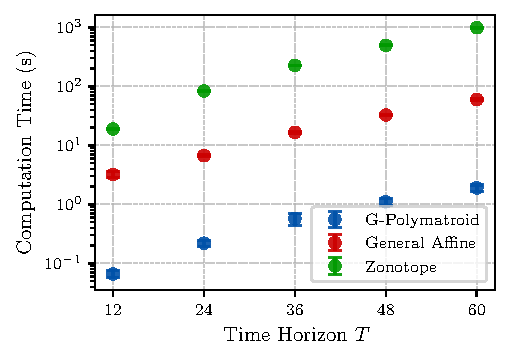
\includegraphics[width=\columnwidth]{./figures/benchmark_plot.pdf}
    \caption{Computation time of various approximation methods to  solve an LP over the aggregate flexibility set of 100 DERs.}
    \label{fig:benchmarking}
  \end{figure}
We first compare the computation time of the proposed aggregation methods against existing benchmarks, considering the \textit{general affine} \cite{Taha2024AnPopulations} and \textit{zonotope-based} \cite{Muller2019AggregationResources} aggregation methods. 
We generate populations of 100 DERs and measure the time each method takes to solve the following LP:
\begin{equation}\label{prob:cost_min}
\begin{aligned}
    \textrm{minimize} \;\; &c^T u \\
    \textrm{s.t.} \;\; &u \in \mathcal{F}(\Xi_{\mathcal{N}}), \quad 
                             Cu \leq d.
\end{aligned}
\end{equation}
where $c\in \mathbb{R}^\mathcal{T}$ denotes the cost vectors of energy over the time horizon and encode network coupling constraints.
This process is repeated for various time horizon lengths, where for each horizon, we generate 100 random instances by independently sampling new populations, network constraints, and energy price profiles. 
The results are plotted in Figure~\ref{fig:benchmarking}, which demonstrate that the proposed methods achieve substantially faster computation times compared to existing approaches in the literature. These findings highlight the scalability and efficiency of the proposed framework, particularly as the problem size and time horizon increase. It is also important to note that the methods from the literature are based on inner approximations of the feasible set, and thus the solutions they produce may be sub-optimal, whereas the proposed methods retain optimality guarantees.


\subsubsection{Case Study}
Finally, we present a case study to illustrate how the proposed aggregation methods can be applied in practice. We consider a population of 50 EVs, half of which have discharging capabilities, and 100 households, each with a load, distributed generation and an ESS. Note that we can aggregate and optimize over larger populations, however the computational limits of the benchmarks we compare against restrict the comparison to the selected population size.
We consider the electricity costs minimization problem from \eqref{prob:cost_min}.
We assess the cost reduction relative to a baseline consumption profile for the population. The baseline consumption profile is defined as follows: each household minimizes their external energy consumption, i.e. minimize the $l_1$ norm of aggregate consumption of the load, distributed generation and the ESS, and the EVs adopt the consumption profile that charges them as soon as possible.
Electricity prices are sampled for each day of November 2022, for the GB system from Elexon \cite{ElexonPortal}, and we sample a new population of devices for each day. 
We compare the performance of the proposed method against the benchmarks introduced in the previous subsection.
In Fig. \ref{fig:case_study} we plot the cumulative cost for the electricity cost minimization problem over the 30 days, for the benchmarks and the baseline cost. Our methods achieve a significant relative cost reduction, compared to the benchmarks for the general affine and zonotope methods.

\begin{figure}[t]
    \centering
    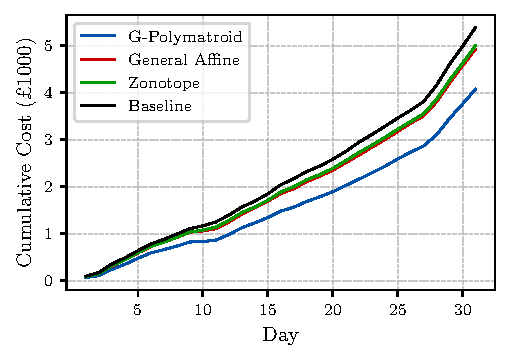
\includegraphics[width=\columnwidth]{./figures/cumulative.pdf}
    \caption{Cumulative electricity cost required to meet the population’s energy demand across the entire month.}
    \label{fig:case_study}
\end{figure}
